\chapter{Execution}

\section{Stating}
\subsection{Commander}
\begin{figure}[H]
	\begin{center}
	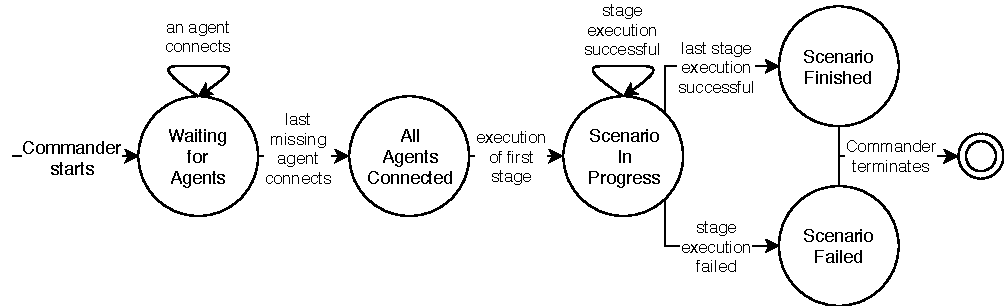
\includegraphics[scale=0.9]{Resources/PDF/CommanderStates}
	\caption{Commander States}
	\label{pic:CommanderStates}
	\end{center}
\end{figure}

\subsection{Agent}
\begin{figure}[H]
	\begin{center}
	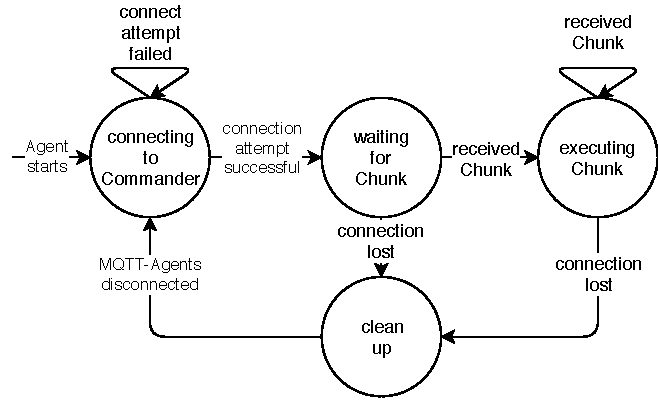
\includegraphics[scale=0.9]{Resources/PDF/AgentStates}
	\caption{Agent States}
	\label{pic:AgentStates}
	\end{center}
\end{figure}

\section{Configuration}
\subsection{Commander}
\begin{lstlisting}[caption={Commander XML configuration}, captionpos=b, label={lst:commanderConfig}, language=XML]
<varroa>
    <commander>
		<bind-host>192.127.0.1</bind-host>
        <bind-port>12345</bind-port>
        <amount-agents>3</amount-agents>
    </commander>
</varroa>
\end{lstlisting}
\begin{itemize}
	\item \textbf{bin-host:} specifies the Address the commander binds to
	\item \textbf{bind-port:} specifies the port the commander binds to for waiting for Agent connections
	\item \textbf{amount-agents:} specifies the amount of Agents that connect to the Commander
\end{itemize}

\subsection{Agent}
\begin{lstlisting}[caption={Agent XML configuration}, captionpos=b, label={lst:agentConfig}, language=XML]
<varroa>
    <agent>
		<commander-host>192.127.0.1</commander-host>
        <commander-port>12345</commander-port>
        <local-port>23458</local-port>
		<commander-retry-interval>10</commander-retry-interval>
    </agent>
</varroa>
\end{lstlisting}
\begin{itemize}
	\item \textbf{commander-port:} specifies the port of the Commander
	\item \textbf{commander-host:} specifies the Address of the Commander
	\item \textbf{local-port:} specifies the local port the Agent uses for the outgoing connection to the Commander %TODO must be different on every Agent
	\item \textbf{commander-retry-interval:} the time interval in which agents try to connect to the commander
\end{itemize}